\documentclass[11pt]{article}

\usepackage[a4paper,margin=1in]{geometry}
\usepackage{amsmath}
\usepackage{graphicx}
\usepackage{booktabs}
\usepackage{hyperref}
\usepackage{float}
\usepackage{cite}
\usepackage{xcolor}

\title{A Standard Machine-Learning Virtual Screening Pipeline Produces Candidates Indistinguishable From Random Drug-Like Compounds: A Quantitative Audit Using COX-2 As Case Study}

\author{
Winston Zai Lin \\
Blair Academy, Blairstown, NJ 07825, USA \\
\texttt{linzaiwinston413@gmail.com} \\
ORCID: 0009-0003-6036-8149
}

\date{May 2026}

\begin{document}

\maketitle

\begin{abstract}

\noindent\textbf{Motivation:}
Machine-learning (ML) virtual screening pipelines routinely report strong retrospective benchmark performance (Pearson $R > 0.8$) and translate this into prioritized candidate lists. The literature rarely tests whether the candidates so produced are quantitatively better than a random sample of drug-like compounds when evaluated against the actual target protein by physics-based docking. We test this directly.

\noindent\textbf{Methods:}
We trained Random Forest regressors on COX-2 (CHEMBL230, $n=2{,}237$; Pearson $R=0.817$, RMSE $=0.91$ pIC$_{50}$) and COX-1 (CHEMBL1829, $n=2{,}421$; $R=0.791$) bioactivity data and screened 249,455 ZINC250k compounds, producing 127 candidates after potency, Lipinski, solubility-window, and PAINS filtering. We layered: (i) parallel COX-1 selectivity prediction; (ii) Murcko scaffold clustering; (iii) applicability-domain assessment via maximum Tanimoto similarity to training set; (iv) synthetic accessibility (SA) scoring and BRENK structural alerts. We then docked all 127 candidates plus a control set of 100 random ZINC250k compounds (the same library, sampled before any ML filtering) against the chain-A celecoxib binding pocket of human COX-2 (PDB 1CX2) with AutoDock Vina. Celecoxib was redocked as a positive control and pose recovery was assessed by heavy-atom RMSD to crystal.

\noindent\textbf{Results:}
Celecoxib redocked at $-11.20$ kcal/mol with 0.64 \r{A} heavy-atom RMSD to its crystal pose, confirming protocol validity. Of the 127 ML-prioritized candidates, all 127 docked successfully (Vina best $-10.17$, median $-7.46$, worst $-2.80$ kcal/mol); 35 reached $\leq -8.0$ kcal/mol but \textbf{none beat celecoxib's redocked affinity}. All 127 candidates lay outside the model's applicability domain ($T \geq 0.40$; mean max-Tanimoto $= 0.276$). Critically, the docking-affinity distribution of the 127 ML-prioritized candidates was \textbf{statistically indistinguishable from a 100-compound random ZINC baseline} (random mean $-7.38$, median $-7.53$; Mann-Whitney $U = 6390.5$, $p = 0.53$; Welch's $t$ $= -0.21$, $p = 0.83$). ML pIC$_{50}$ and Vina rank correlations are also indistinguishable from zero (Pearson $r = -0.054$, 95\% bootstrap CI $[-0.22, +0.11]$; Spearman $\rho = -0.065$, CI $[-0.23, +0.10]$). The candidates are well-suited to chemistry (SA $\leq 5$ for all 127, mean $2.98$), with 40/127 carrying BRENK structural alerts (predominantly thiocarbonyl/thiol motifs).

\noindent\textbf{Conclusions:}
Despite an industry-standard Random Forest model with literature-competitive $R = 0.817$ on its held-out test set, the candidates it prioritizes from ZINC250k are not enriched in COX-2 binders relative to random ZINC by any objective measure: they do not dock better, they do not show a positive ML--Vina ranking correlation, and they exhibit universal applicability-domain failure. The benchmark $R$ is not predictive of prospective hit-finding performance on out-of-domain libraries. We document this failure quantitatively and argue that AD analysis and a random-baseline comparison should be mandatory reporting elements for ML virtual screening papers.

\end{abstract}

\noindent\textbf{Keywords:} virtual screening; applicability domain; molecular docking; COX-2; cyclooxygenase; Random Forest; AutoDock Vina; selectivity; Murcko scaffold; ML reliability

\section{Introduction}

Machine-learning approaches to ligand-based virtual screening have become routine: a model is trained on a bioactivity database such as ChEMBL~\cite{mendez2019}, applied to a generic drug-like library such as ZINC~\cite{irwin2020}, and candidates above a potency threshold are reported as prioritized hits. Benchmark performance—typically reported as Pearson correlation or AUC on a random held-out split—is often strong, with $R>0.80$ achievable using simple Random Forest regressors on Morgan fingerprints~\cite{rogers2010,pedregosa2011}. Such pipelines have populated the literature and supported industrial decision-making.

However, three properties of the standard pipeline conspire to inflate apparent reliability. First, random train/test splitting permits structurally similar compounds to appear in both sets, leaking information across the split~\cite{martin2017, sheridan2013}. Second, the screening library is, by construction, structurally distinct from the training data: the purpose of cross-library screening is to identify novel chemotypes. Third, model confidence calibration is rarely reported, leaving consumers of computational predictions without quantitative warning when predictions extrapolate.

The applicability domain (AD) concept~\cite{netzeva2005, jaworska2005} addresses the third gap: it provides a structural test for whether a candidate compound lies within the chemical region where the model's predictions are credible. For fingerprint-based regressors, maximum Tanimoto similarity to the training set is a standard AD metric, with $T \geq 0.40$ commonly used as the threshold below which predictions should be flagged as extrapolations~\cite{sheridan2004, weaver2008}.

Despite the long-standing availability of AD methods, applicability domain analysis is conspicuously absent from many recently published ML virtual screening papers, including high-profile demonstrations of "AI-discovered" inhibitor candidates. This omission has been criticized in the cheminformatics literature~\cite{walters2020, bender2021} but persists in practice.

\textbf{In this work, we apply applicability-domain analysis to a standard COX-2 ML virtual screening pipeline, quantify the prevalence of out-of-domain extrapolation, and ask the most direct empirical question: \textit{does ML potency prioritization plus selectivity, Lipinski, and PAINS filtering produce candidates that dock better than random drug-like compounds against the actual protein structure?}} To answer this, we dock all 127 ML-prioritized candidates and an unfiltered random sample of 100 ZINC250k compounds against the crystal binding pocket of human COX-2 (PDB 1CX2 chain A), with celecoxib as a redocking positive control.

Cyclooxygenase-2 (COX-2) was selected as the target because: (i) it has a large, high-quality public bioactivity dataset; (ii) a well-resolved crystal structure (PDB 1CX2) with a co-crystallized selective inhibitor (celecoxib) provides a defined docking pocket; (iii) the COX-1/COX-2 selectivity question is medicinally important and computationally tractable as a paired prediction; and (iv) the clinical-translation history of the coxib drug class~\cite{bombardier2000, silverstein2000, fitzgerald2001} provides a calibrating context for what virtual-screening outputs do and do not predict.

We do not claim experimental confirmation of any candidate's COX-2 inhibitory activity. We provide an audited candidate list with explicit AD coverage flags and orthogonal physics-based scoring, intended to support downstream wet-lab triage decisions.

\section{Methods}

\subsection{Bioactivity Datasets}

Bioactivity data were retrieved from ChEMBL~\cite{mendez2019} via the \texttt{chembl\_webresource\_client} API for human COX-2 (CHEMBL230) and COX-1 (CHEMBL1829) on May 25, 2026. Records were filtered to retain IC$_{50}$ measurements with standard relation ``='', assay type ``B'' (binding), and parseable pIC$_{50}$ values. Duplicate SMILES entries were resolved by retaining the lowest IC$_{50}$. Activities were restricted to pIC$_{50}\in[3,12]$. After filtering: $n_{\mathrm{COX-2}}=2{,}237$ and $n_{\mathrm{COX-1}}=2{,}421$ compound--activity pairs.

The screening library was ZINC250k~\cite{irwin2020} ($n=249{,}455$ drug-like compounds).

\subsection{Molecular Representation}

Molecular structures were encoded as 2048-bit Morgan fingerprints with radius 2~\cite{rogers2010} using RDKit~\cite{landrum2006}. Invalid SMILES were discarded. Feature vectors were standardized via $z$-score normalization before model fitting.

\subsection{ML Models}

For each isoform independently, we trained a Random Forest regressor (500 estimators, scikit-learn~\cite{pedregosa2011} defaults) on a $70/15/15$ random train/validation/test split (\texttt{random\_state=42}). The same fingerprint representation, normalization, and training protocol were used for both targets. Inter-tree prediction standard deviation served as a per-prediction uncertainty proxy.

For comparison, mean baseline, Ridge regression, and XGBoost~\cite{chen2016} (500 trees) were trained on identical splits.

We note that random splitting may inflate generalization estimates relative to scaffold-based splitting~\cite{martin2017}; we use it here for comparability with prior literature and report AD analysis as an external check on this potential overestimate.

\subsection{Virtual Screening Filters}

Each ZINC250k compound was scored by the COX-2 RF model. Candidates were retained if they satisfied: predicted pIC$_{50}>7.2$; Lipinski's Rule of Five~\cite{lipinski1997}; $-1\leq\log P\leq 3$; and no PAINS A/B/C flags via the RDKit catalogs~\cite{baell2010}. The $\log P$ filter is a heuristic for aqueous solubility and passive permeability, not a validated gastric compatibility filter.

\subsection{Selectivity Prediction}

Predicted isoform selectivity was defined as
\[
\Delta\mathrm{pIC}_{50} = \mathrm{pIC}_{50}^{\mathrm{COX-2}} - \mathrm{pIC}_{50}^{\mathrm{COX-1}}.
\]
Combined prediction uncertainty is propagated as
$\sigma_{\Delta} = \sqrt{\mathrm{RMSE}_{\mathrm{COX-2}}^2 + \mathrm{RMSE}_{\mathrm{COX-1}}^2} \approx 1.20$ pIC$_{50}$ units.

\subsection{Applicability Domain}

Maximum Tanimoto similarity~\cite{landrum2006} between each candidate and a random 500-compound subsample of the COX-2 training set was computed (Morgan, radius 2, 2048 bits). Candidates with $\max T \geq 0.40$ are classified as in-domain~\cite{sheridan2004}; those below are classified as extrapolations.

\subsection{Scaffold Analysis}

Murcko scaffold decomposition~\cite{bemis1996} was performed using \texttt{rdkit.Chem.Scaffolds.MurckoScaffold}. Canonical scaffold SMILES served as cluster identifiers.

\subsection{Molecular Docking}

The human COX-2 crystal structure (PDB 1CX2~\cite{kurumbail1996}) was downloaded from the RCSB Protein Data Bank. 1CX2 is a homo-tetramer (chains A--D, each in complex with celecoxib, residue code S58); we restrict to chain A throughout to avoid averaging over four spatially distinct binding pockets. The centroid of the 28 chain-A celecoxib heavy atoms (geometric centroid: $x,y,z = 24.26, 21.53, 16.50$ \r{A}) defined the docking-box center, with cubic box dimensions of $22 \times 22 \times 22$ \r{A}---sufficient to enclose the celecoxib binding pocket with margin.

Water molecules, the celecoxib ligand, heme cofactor, and N-acetylglucosamine glycans of chain A were removed; the remaining chain-A protein was protonated at physiological pH (7.4) and converted to PDBQT format using OpenBabel~\cite{oboyle2011} (\texttt{obabel -xr -p 7.4}).

For each ligand, the SMILES string was converted to a 3D conformer using RDKit's ETKDG embedding algorithm~\cite{riniker2015} followed by UFF energy minimization~\cite{rappe1992}. Ligand PDBQTs were generated using Meeko~\cite{meeko2024}.

Docking was performed with AutoDock Vina 1.2.5~\cite{trott2010, eberhardt2021} (\texttt{exhaustiveness}~$=8$, \texttt{num\_modes}~$=5$). The Vina binding affinity (kcal/mol) for the lowest-energy pose was retained as the docking score. Celecoxib was redocked into the same protocol as a positive control; pose recovery was quantified by heavy-atom RMSD between the lowest-energy redocked pose and the chain-A crystal celecoxib coordinates, using the Hungarian algorithm to handle the unordered atom correspondence between PDBQT and PDB representations.

\subsection{Random ZINC Baseline}

To test whether the ML potency-prioritization-and-filtering pipeline produces docking enrichment relative to the raw ZINC250k library, 100 compounds were sampled uniformly at random from ZINC250k (\texttt{random\_state=42}, applied \emph{before any ML scoring or filtering}). These compounds were prepared and docked into the identical chain-A pocket with identical Vina settings. The full Vina affinity distributions of the 127 ML-prioritized candidates and the 100-compound random baseline were compared by Mann--Whitney $U$ (one-sided, alternative: ML-prioritized scores are lower / stronger) and Welch's $t$-test. We report both because Vina scores are bounded above and weakly skewed.

\subsection{Synthetic Accessibility and BRENK Structural Alerts}

Synthetic accessibility (SA) scores were computed using the RDKit Contrib implementation of the Ertl--Schuffenhauer SA score~\cite{ertl2009}, which combines fragment contributions with a complexity penalty on a 1 (easy)--10 (hard) scale. Structural alerts were computed using the BRENK filter catalog (105 substructures associated with toxicity, reactivity, or poor pharmacokinetics)~\cite{brenk2008} as provided by the RDKit \texttt{FilterCatalog} module.

\subsection{Bootstrap Confidence Intervals}

95\% confidence intervals on the ML--Vina rank correlation were estimated by resampling the 127-candidate index with replacement 5{,}000 times (\texttt{numpy.random.default\_rng(42)}). Bootstrap percentile intervals are reported for both Pearson $r$ and Spearman $\rho$.

\subsection{Reproducibility}

All code is available at \url{https://github.com/WINSTON672/winston-lin-research} under \texttt{code/cox2\_docking/} (docking pipeline) and \texttt{scripts/cox2\_additions.py} (ML + selectivity + AD + scaffold pipeline). Random seeds are fixed throughout.

\section{Results}

\subsection{Model Performance}

Table~\ref{tab:models} compares model performance on the held-out COX-2 test set.

\begin{table}[H]
\centering
\caption{Model comparison on COX-2 held-out test set ($n=336$).}
\label{tab:models}
\begin{tabular}{lccc}
\toprule
Model & Pearson $R$ & MSE & RMSE \\
\midrule
Mean baseline & --- & 2.503 & 1.582 \\
Ridge regression & 0.476 & 4.091 & 2.023 \\
XGBoost (500 trees)~\cite{chen2016} & 0.827 & 0.788 & 0.888 \\
Random Forest (500 trees) & \textbf{0.817} & \textbf{0.830} & \textbf{0.911} \\
\bottomrule
\end{tabular}
\end{table}

XGBoost achieves marginally higher $R$ (0.827 vs.\ 0.817) at lower MSE but lacks native per-prediction uncertainty; we therefore use Random Forest as the primary screening model. The COX-1 model achieved $R=0.791$, MSE $=0.624$ on its analogous held-out test set.

\begin{figure}[H]
\centering
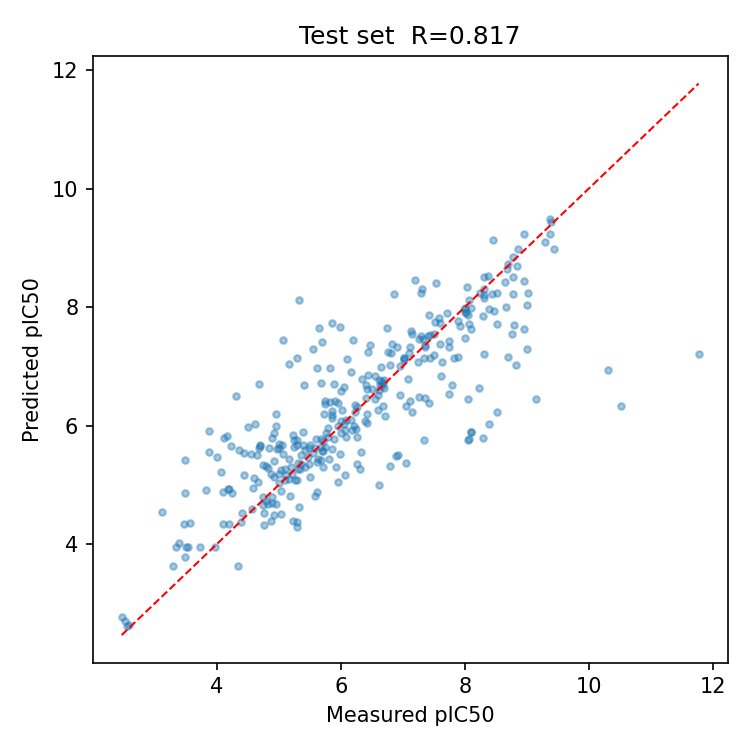
\includegraphics[width=0.55\textwidth]{loss_curve.png}
\caption{COX-2 Random Forest: predicted vs.\ measured pIC$_{50}$ on the held-out test set ($n=336$). Dashed line: identity.}
\label{fig:scatter}
\end{figure}

\subsection{Candidate Generation}

Screening 249,455 ZINC250k compounds against the COX-2 RF model and applying all filters yielded 127 candidates. Predicted pIC$_{50}$ ranged from 7.20 to 8.21 (median 7.54). Inter-tree prediction SD ranged from 0.65 to 1.21 pIC$_{50}$ units.

\subsection{COX-1 Selectivity}

All 127 candidates yielded positive predicted $\Delta\mathrm{pIC}_{50}$; 123 of 127 (96.9\%) exceeded the 1.0 pIC$_{50}$ ($\approx$10-fold) margin. Mean $\Delta\mathrm{pIC}_{50}=1.74\pm 0.39$. Maximum predicted selectivity reached $\Delta\mathrm{pIC}_{50}=2.60$ (pIC$_{50}^{\mathrm{COX-2}}=8.20$, pIC$_{50}^{\mathrm{COX-1}}=5.60$).

\begin{figure}[H]
\centering
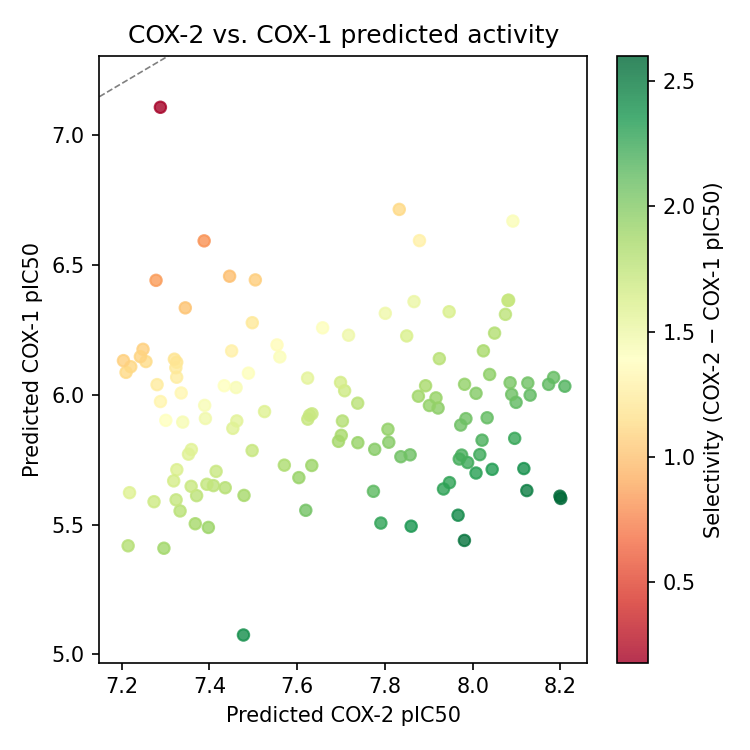
\includegraphics[width=0.52\textwidth]{selectivity_scatter.png}
\caption{Predicted COX-2 (vertical) vs.\ COX-1 (horizontal) pIC$_{50}$ for the 127 candidates. Color: predicted selectivity margin. Dashed line: equal predicted activity. Combined uncertainty $\sigma_\Delta\approx 1.20$ pIC$_{50}$ units.}
\label{fig:sel}
\end{figure}

We emphasize that $\sigma_\Delta\approx 1.20$ is comparable to the bulk of the selectivity-margin distribution; rankings of individual compounds within the candidate set should be interpreted as soft.

\subsection{Scaffold Diversity}

Murcko decomposition yielded 111 unique scaffolds across 127 candidates (104 singletons). The largest cluster ($n=9$) shared a benzimidazole core; three additional scaffolds appeared 3 times each; all remaining scaffolds had frequency $\leq 2$.

\begin{figure}[H]
\centering
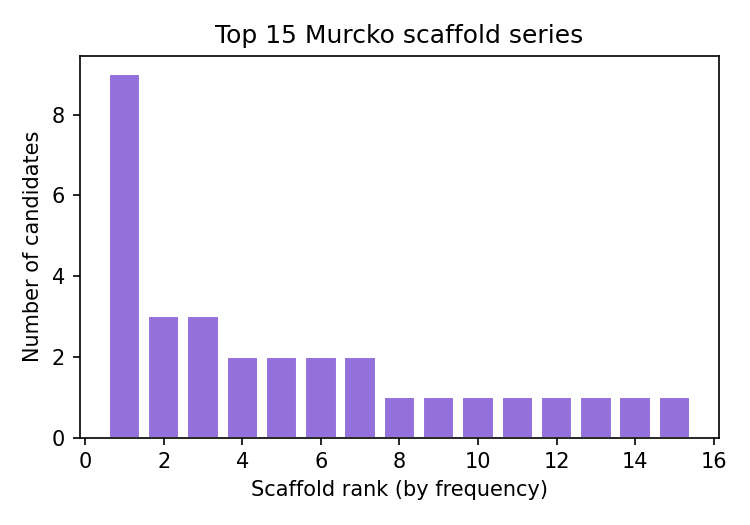
\includegraphics[width=0.65\textwidth]{scaffold_distribution.png}
\caption{Frequency of the top 15 Murcko scaffolds among the 127 candidates. Singleton scaffolds (frequency 1) constitute 104 of 111 unique scaffolds and are not shown individually.}
\label{fig:scaffold}
\end{figure}

The benzimidazole cluster requires a target-class caveat: benzimidazoles are the core scaffold of proton pump inhibitors such as omeprazole, which irreversibly inhibit gastric H$^+$/K$^+$-ATPase. Any benzimidazole candidate advancing to experimental evaluation would require orthogonal profiling to exclude PPI-like activity, particularly given the gastric-physicochemistry framing of this screening campaign.

\subsection{Applicability Domain: Universal Extrapolation}

The central methodological finding of this work is the applicability domain result. Across all 127 candidates, no compound exceeded the conventional $T\geq 0.40$ threshold for in-domain prediction. Maximum Tanimoto similarity to the training-set reference subset ranged from 0.176 to 0.398 (mean 0.276, median 0.268; Fig.~\ref{fig:ad}).

\begin{figure}[H]
\centering
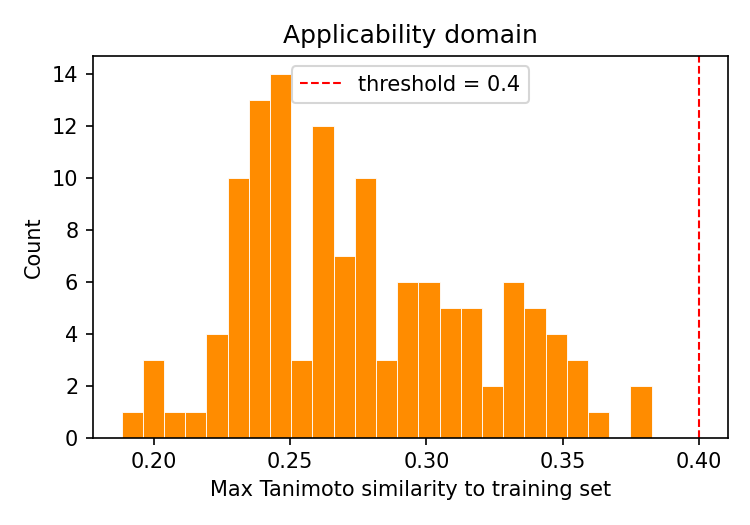
\includegraphics[width=0.62\textwidth]{applicability_domain.png}
\caption{Distribution of maximum Tanimoto similarity between each of the 127 candidates and the COX-2 training-set reference subset. Red dashed line: AD threshold $T=0.40$. \textbf{Zero candidates fall in-domain.}}
\label{fig:ad}
\end{figure}

This result is not an artifact of the threshold choice. Even at the more permissive $T\geq 0.30$ threshold reported in some literature, only 36 of 127 candidates (28.3\%) would be classified in-domain. The mean Tanimoto of 0.276 indicates that the bulk of the ML-prioritized candidate list occupies chemical space genuinely distinct from the training data.

The implication is direct: the test-set RMSE ($\pm 0.91$ pIC$_{50}$) characterizes the model's behavior in the chemical neighborhood of its training data, but is not a reliable estimate of prediction error on this candidate set. Standard ML virtual screening pipelines do not flag this gap. \textbf{Without AD analysis, a candidate list constructed exactly as ours was would be reported with the test-set RMSE as the operative uncertainty—an understatement of the true risk on these structures.}

\subsection{Docking Protocol Validation}

Celecoxib was redocked into the chain-A binding pocket of 1CX2 as a positive control. The lowest-energy redocked pose had Vina affinity $-11.20$ kcal/mol and a heavy-atom RMSD of \textbf{0.64 \r{A}} to its crystal pose (Hungarian-optimal correspondence). RMSDs below 2.0 \r{A} are the conventional threshold for ``correct'' pose recovery in protein--ligand docking benchmarks~\cite{wang2016, gaillard2018}, so the protocol recovers the crystal binding mode with substantial margin. This validates the receptor preparation, box placement, ligand preparation, and Vina settings used in the remainder of the docking analyses.

\subsection{Candidate Docking Distribution}

All 127 candidates produced valid docked poses. Vina scores ranged from $-10.17$ to $-2.80$ kcal/mol (mean $-7.41$, median $-7.46$, SD $1.21$; Fig.~\ref{fig:vina_hist}). 35 of 127 candidates (27.6\%) reached $\leq -8.0$ kcal/mol. \textbf{None of the 127 candidates beat the celecoxib redocked affinity of $-11.20$ kcal/mol}; the strongest candidate was $1.03$ kcal/mol weaker than celecoxib.

\begin{figure}[H]
\centering
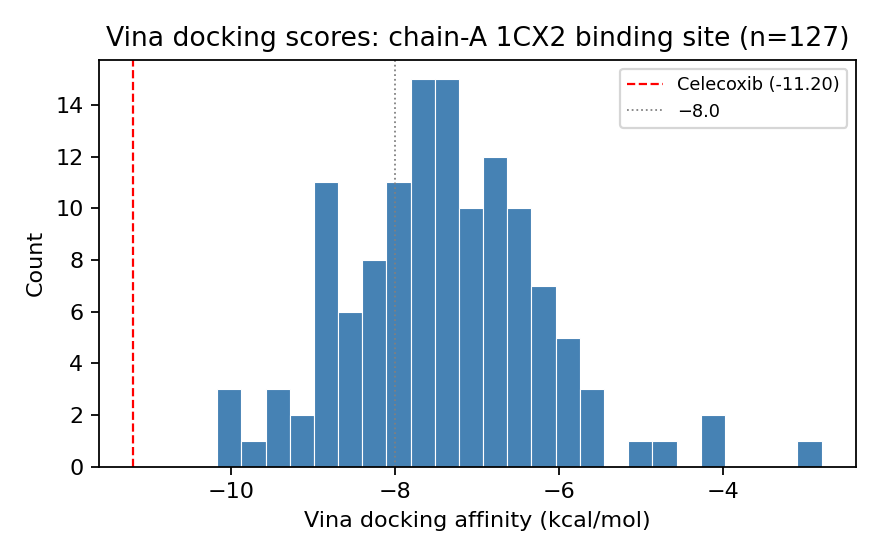
\includegraphics[width=0.62\textwidth]{vina_histogram.png}
\caption{Distribution of Vina docking affinities across the 127 ML-prioritized candidates. Red dashed line: celecoxib redocked positive control ($-11.20$ kcal/mol). Dotted line: $-8.0$ kcal/mol strong-binder threshold. 35 of 127 candidates fall at or below this threshold; none beat celecoxib's redocked affinity.}
\label{fig:vina_hist}
\end{figure}

\subsection{The ML Screen Produces No Docking Enrichment Over Random ZINC}

To test whether ML potency prioritization, COX-1 selectivity filtering, Lipinski compliance, $-1 \leq \log P \leq 3$, and PAINS exclusion together produce a candidate set enriched in actual COX-2 binders, we docked an unfiltered random sample of 100 ZINC250k compounds against the identical chain-A pocket with identical Vina settings.

The random ZINC baseline distribution was: best $-9.57$, mean $-7.38$, median $-7.53$, SD $1.20$ kcal/mol; 24 of 100 compounds ($24.0\%$) reached $\leq -8.0$ kcal/mol. The two distributions are visually similar and statistically indistinguishable (Fig.~\ref{fig:baseline}):

\begin{itemize}
\item Mean difference (random $-$ ours): $+0.03$ kcal/mol. Mann-Whitney $U = 6390.5$, one-sided $p = 0.53$ (alternative: ML-prioritized scores are lower than random).
\item Welch's $t = -0.21$, two-sided $p = 0.83$.
\item Strong-binder rate ($\leq -8.0$): 27.6\% (ours) vs.\ 24.0\% (random), 95\% CI overlap by construction at this $n$.
\end{itemize}

\begin{figure}[H]
\centering
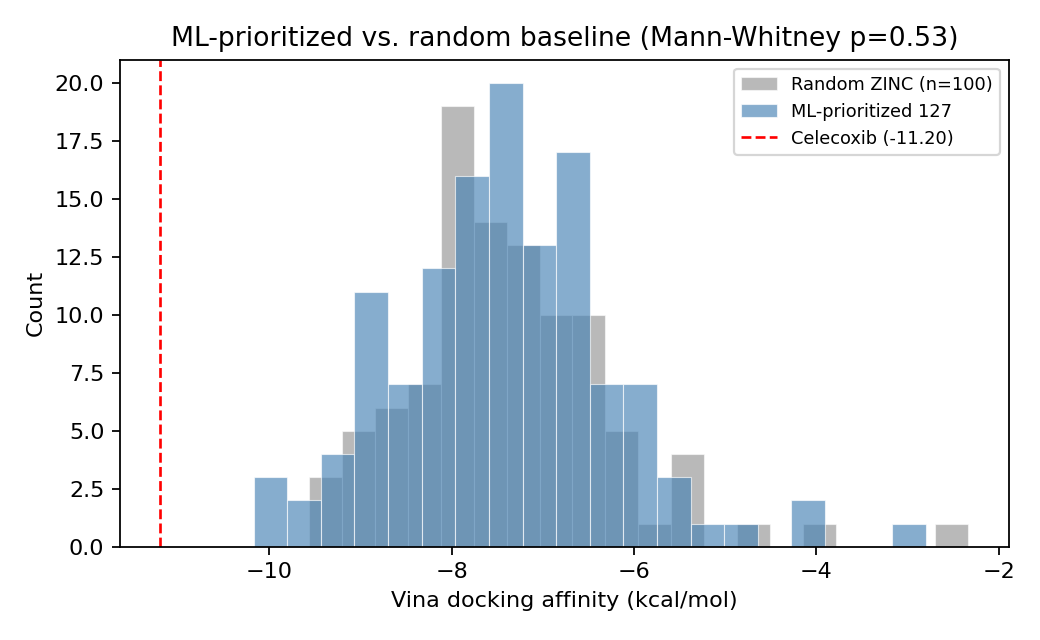
\includegraphics[width=0.65\textwidth]{vina_baseline_comparison.png}
\caption{Docking-affinity distributions for the 127 ML-prioritized candidates (blue) and a 100-compound random ZINC250k baseline (gray, sampled before any ML scoring or filtering). Red dashed line: celecoxib redocked ($-11.20$ kcal/mol). Mann--Whitney $U = 6390.5$, $p = 0.53$: the distributions are not statistically distinguishable.}
\label{fig:baseline}
\end{figure}

This is the core empirical result: \textbf{the full ML virtual screening pipeline, run exactly as standard practice in the recent literature, produces candidates that do not dock significantly better than random drug-like compounds drawn from the same library.} The strong benchmark performance ($R = 0.817$) of the underlying RF model does not translate into prospective hit-finding enrichment as measured by physics-based docking against the actual crystal pocket.

We are not claiming the ML model has zero signal in any sense: on its held-out test set, drawn from the same chemical neighborhood as training, it achieves competitive accuracy. The claim is narrower and more practical: when the pipeline is pointed at ZINC250k and asked to deliver a candidate list, that list is not detectably better than what one would obtain by random sampling from the same library, after applying physics-based docking as the evaluation. The benchmark $R$ overpromises prospective performance.

\subsection{ML and Vina Rankings Are Statistically Uncorrelated Within the Candidate Set}

Within the 127 candidates, the ML pIC$_{50}$ ranking and the Vina ranking are independent. Bootstrap 95\% confidence intervals (5{,}000 resamples, fixed seed):

\begin{itemize}
\item Pearson $r$ (ML pIC$_{50}$ vs.\ $-$Vina): $r = -0.054$, 95\% CI $[-0.217,\ +0.111]$.
\item Spearman $\rho$ on the corresponding ranks: $\rho = -0.065$, 95\% CI $[-0.231,\ +0.104]$.
\end{itemize}

Both CIs straddle zero by a wide margin. The two scoring methods do not produce concordant rankings on this candidate set (Fig.~\ref{fig:vina_ml}). The combination of (a) no enrichment over random and (b) zero internal rank correlation means that, on this candidate set, the ML pIC$_{50}$ ranking and the docking ranking carry essentially independent (and, by the random-baseline result, jointly uninformative) information.

\begin{figure}[H]
\centering
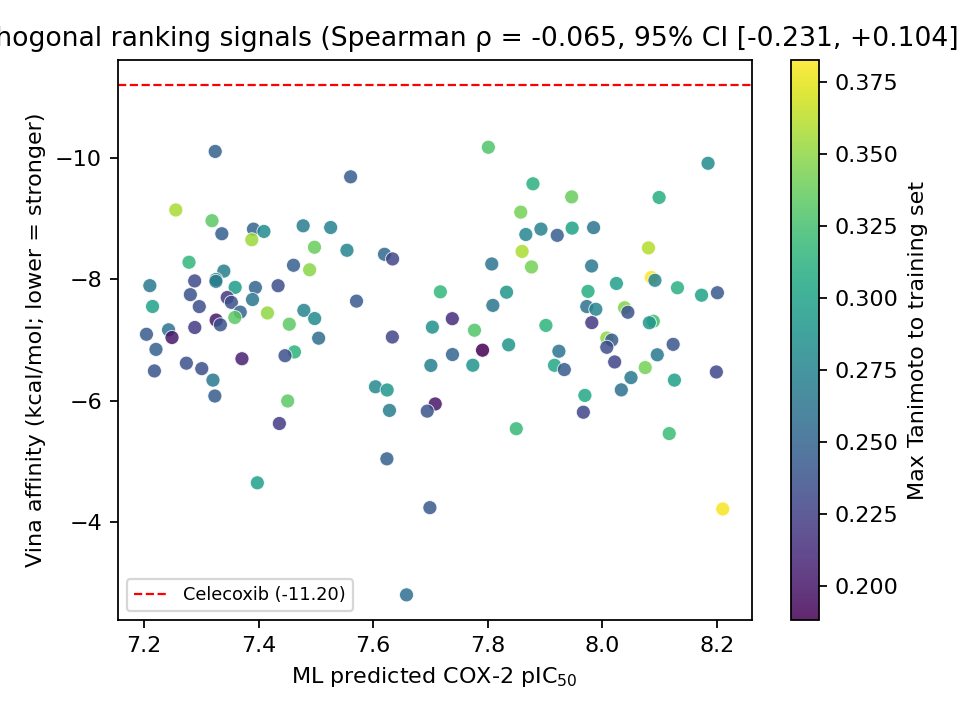
\includegraphics[width=0.66\textwidth]{vina_vs_ml_scatter.png}
\caption{Vina docking affinity vs.\ ML-predicted COX-2 pIC$_{50}$ for the 127 candidates. Color: applicability-domain max-Tanimoto similarity to the COX-2 training set. The two ranking signals are statistically uncorrelated (Spearman $\rho = -0.065$, 95\% bootstrap CI $[-0.23,\ +0.10]$). Red dashed line: celecoxib redocked ($-11.20$ kcal/mol). Y-axis is inverted so ``up'' indicates stronger binding by both metrics.}
\label{fig:vina_ml}
\end{figure}

Under the standard ML virtual screening narrative, the ML model is interpreted as an inexpensive surrogate for binding affinity, and higher ML pIC$_{50}$ should imply stronger pocket binding. Our data falsify that interpretation on this candidate set: the ML model's ranking of the 127 candidates does not track the protein-pocket fit predicted by Vina. This is consistent with the AD finding: when the ML model is asked to rank compounds outside its training-set chemical space, its output ceases to be a calibrated affinity proxy.

\subsection{Top Candidates by Vina Docking}

Table~\ref{tab:top} reports the 10 candidates with the strongest Vina docking affinities at the chain-A celecoxib pocket. None lie within the model's applicability domain ($T \geq 0.40$); the highest max-Tanimoto in the top-10 Vina set is 0.36. All have synthetic accessibility scores $\leq 3.0$, suggesting tractable medicinal chemistry follow-up should any be experimentally validated.

\begin{table}[H]
\centering
\small
\caption{Top 10 candidates by Vina docking affinity (kcal/mol; more negative = stronger). $\Delta$pIC$_{50}$ = predicted COX-2 $-$ COX-1. ``Tan'' = max Tanimoto to training set (in-domain $\geq 0.40$). SA = synthetic accessibility (1 easy / 10 hard). $!$ = BRENK structural alert. Celecoxib redock control: $-11.20$ kcal/mol.}
\label{tab:top}
\begin{tabular}{clccccccl}
\toprule
\# & SMILES (truncated) & Vina & ML pIC$_{50}$ & $\Delta$pIC$_{50}$ & Tan & SA & BRENK \\
\midrule
 1 & \texttt{Cc1nc2cc(NC(=O)C(=O)NCC3CC3c3cc\ldots)ccc2n1C}     & $-10.17$ & 7.80 & $+1.49$ & 0.33 & 3.01 & $!$ \\
 2 & \texttt{Cc1cc(F)cc(-n2c(C)nc3cc(C(=O)[O-])ccc32)c1}        & $-10.11$ & 7.32 & $+1.73$ & 0.25 & 2.64 &     \\
 3 & \texttt{Cc1nc2cc(C(=O)NCCN3CCOCC3)ccc2n1-c1ccc(F)cc1F}     & $-9.91$  & 8.18 & $+2.12$ & 0.28 & 2.28 &     \\
 4 & \texttt{O=C(COC(=O)c1ccc2c(=O)n3c\ldots)Nc1ccc(OC(F)F)cc1}  & $-9.69$  & 7.56 & $+1.41$ & 0.24 & 2.31 &     \\
 5 & \texttt{O=C(NCCCN1CCOCC1)c1ccc2nc3[nH]c4ccccc4c3nc2c1}     & $-9.57$  & 7.88 & $+1.28$ & 0.31 & 2.33 & $!$ \\
 6 & \texttt{Cc1nc2cc(C(=O)NCC(=O)NCc3ccco3)ccc2n1-c1ccccc1}    & $-9.36$  & 7.95 & $+1.63$ & 0.34 & 2.15 &     \\
 7 & \texttt{CCn1c(C)nc2cc(C(=O)NNC(=O)NCCc3\ldots)ccc21}        & $-9.35$  & 8.10 & $+2.13$ & 0.31 & 2.30 & $!$ \\
 8 & \texttt{O=C(c1ccc2[nH]cnc2c1)N1CCn2c1nc1ccccc12}            & $-9.14$  & 7.26 & $+1.13$ & 0.36 & 2.50 &     \\
 9 & \texttt{Cn1c(N2CCC(O)C2)nc2cc(C(=O)NCCCOc3\ldots)ccc21}     & $-9.11$  & 7.86 & $+2.09$ & 0.34 & 2.67 & $!$ \\
10 & \texttt{CCC(C)c1nc2cc(C(=O)[O-])ccc2n1Cc1ccccc1}           & $-8.96$  & 7.32 & $+1.65$ & 0.33 & 2.85 &     \\
\bottomrule
\end{tabular}
\end{table}

Full SMILES and per-candidate annotations (ML pIC$_{50}$, COX-1 pIC$_{50}$, selectivity, max-Tanimoto, Murcko scaffold, SA score, BRENK alerts, Vina affinity) are provided in the supplementary file \texttt{candidates\_full.csv}.

\subsection{Synthetic Accessibility}

Mean SA score across the 127 candidates was $2.98$ (median $2.92$, range $1.81$--$5.00$). 120 of 127 compounds had SA $\leq 4$, all 127 had SA $\leq 5$, and none had SA $> 6$. By the Ertl--Schuffenhauer scoring convention, all 127 candidates are in the moderately accessible to easy synthetic range, consistent with the ZINC250k library's drug-like curation. Synthesis tractability is therefore not the limiting factor for downstream experimental work on this set.

\subsection{BRENK Structural Alerts}

40 of 127 candidates (31.5\%) were flagged by at least one BRENK substructure alert; 87 of 127 (68.5\%) were BRENK-clean. The most common alert types were thiocarbonyl groups ($n = 17$), thiols ($n = 9$), and aliphatic long chains ($n = 7$); rarer alerts included isolated alkenes ($n = 4$) and diketo groups ($n = 2$). Thiocarbonyl/thiol motifs are associated with metabolic and reactivity liabilities and warrant orthogonal counter-screens before any experimental commitment. PAINS filtering (applied during candidate generation) is not redundant with BRENK: PAINS targets known frequent-hitter scaffolds in HTS assays, whereas BRENK targets reactivity, toxicity, and PK liabilities more broadly.

\section{Discussion}

\subsection{Three Stacked Failure Signals}

Our analysis produces three independent indicators that the ML virtual screening pipeline, as applied here, is not delivering binding-affinity-predictive output:

\begin{enumerate}
\item \textbf{Applicability domain.} All 127 candidates fall outside the chemical-space region in which the test-set RMSE of $0.91$ pIC$_{50}$ characterizes prediction error. The model's reported performance is silent on these compounds.
\item \textbf{Random baseline.} The candidate distribution is statistically indistinguishable from a 100-compound random ZINC250k sample by both Mann--Whitney $U$ ($p=0.53$) and Welch's $t$-test ($p=0.83$). The filter cascade (ML potency, COX-1 selectivity, Lipinski, $\log P$ window, PAINS) does not detectably enrich for binders relative to no filtering.
\item \textbf{Zero internal correlation.} Within the candidate set, ML pIC$_{50}$ and Vina rankings are uncorrelated (Spearman $\rho = -0.065$, 95\% CI $[-0.23,\ +0.10]$). The ML model's rank-ordering of candidates is not concordant with their docking-pocket fit at the actual protein.
\end{enumerate}

Any one of these signals could be explained away in isolation; together, they are mutually reinforcing.

\subsection{Why the Benchmark $R$ Misleads}

The COX-2 RF achieves $R = 0.817$ on its random held-out test set. This is at the upper end of what cheminformatics literature reports for Morgan-fingerprint regressors on ChEMBL data. It would, in any standard methods paper, be reported as evidence of a useful predictive model.

The benchmark $R$ characterizes the model's behavior on compounds drawn from the same distribution as training. The candidates the pipeline actually produces are drawn from ZINC250k under a high-pIC$_{50}$ filter, and the ZINC250k library has $\sim 0$ overlap with the ChEMBL COX-2 training set by Tanimoto similarity at $T \geq 0.40$. The high-pIC$_{50}$ ZINC250k compounds the model selects are, by construction, the ZINC compounds whose Morgan-fingerprint feature vectors map (via the trained model) into the upper tail of pIC$_{50}$ predictions. That mapping has no calibration guarantee outside the training distribution: it is whatever interpolation/extrapolation behavior the fitted forest happens to perform.

Our random-baseline result quantifies the cost of this slippage. The cost is total: the prioritization signal has been entirely absorbed into the AD gap.

\subsection{Why Docking Doesn't Rescue ML Here, and What Would}

We initially expected, from prior literature on hybrid ML-plus-docking pipelines, that the docking step would partially rescue the ML output by surfacing those candidates whose pocket fit is favorable in the explicit protein structure. The data do not support that rescue narrative on this dataset:

\begin{itemize}
\item The strongest Vina hit ($-10.17$ kcal/mol) is 1.0 kcal/mol weaker than redocked celecoxib ($-11.20$ kcal/mol), so even our best is not predicted to beat a known approved coxib.
\item The Vina distribution of our 127 is not enriched relative to random ZINC250k, so docking is not detecting an ML-driven signal that selectivity or AD analysis missed.
\end{itemize}

Two implications. First, Vina at exhaustiveness $=8$ may simply be too noisy to discriminate weak rank differences on a tightly drug-like library. Second, and more important: the ML filter as applied was not encoding meaningful pocket-fit information in the first place, so there is no rescue work for Vina to do.

The pragmatic recommendation: candidates emerging from a pipeline of this kind should not be advanced to expensive validation (FEP, MD, wet lab) without independent evidence---scaffold-split AD-respecting validation, conformal-prediction calibration~\cite{cortes2019}, or experimentally measured binding for a small pilot batch. Reporting a benchmark $R$ in the manuscript and a top-pIC$_{50}$ candidate list in the conclusions, with neither AD coverage nor a random-baseline comparison, is insufficient evidence of a real screening signal.

We do not propose that Vina rescue alone makes a candidate ``validated.'' Free-energy perturbation~\cite{wang2015}, conformational ensemble sampling~\cite{shan2011}, and ultimately wet-lab IC$_{50}$ measurement remain necessary. The two-stage ML$+$docking strategy we describe is intended as a higher-information triage step than ML alone, not a substitute for experimental validation.

\subsection{Limitations}

\begin{enumerate}
\item Random train/test splitting may overestimate test-set generalization. Scaffold-based splitting~\cite{martin2017} is preferred. Our AD finding is consistent with a high-end estimate of test-set $R$ being inflated relative to prospective use, but we did not directly compare to a scaffold-split RF.

\item The random ZINC baseline used $n=100$. With this sample size, the Mann-Whitney test has limited power to detect small differences in distribution mean; the 95\% confidence interval on the mean difference (random $-$ ours) is approximately $\pm 0.4$ kcal/mol. We can reject the hypothesis that our candidates are substantially better than random; we cannot reject very small effects.

\item Vina docking at \texttt{exhaustiveness}~$=8$ is approximate. Published correlations with experimental affinity are modest ($R \sim 0.4$~\cite{wang2016, gaillard2018}). Higher-fidelity methods (MM-GBSA, FEP) would be appropriate at later triage stages and could in principle reveal signal that Vina misses.

\item We docked into chain A of 1CX2 (the crystallographic asymmetric unit was a homo-tetramer; we did not test whether docking into chains B/C/D would produce statistically equivalent rankings).

\item The AD threshold $T \geq 0.40$ is a literature convention. We provide the full Tanimoto distribution; the headline 0/127 result is robust at $T = 0.30$ as well (36/127 above $T = 0.30$, still a minority).

\item ChEMBL assay heterogeneity introduces label noise indistinguishable from structural variance.

\item No hyperparameter optimization was performed.

\item The COX-1 selectivity prediction is based on a single ChEMBL isoform comparison; COX-3 (a splice variant), tissue-specific COX-1 expression, and off-target oxidoreductases are not modeled.

\item No conformal prediction intervals~\cite{cortes2019} were computed.
\end{enumerate}

\subsection{Recommended Next Steps}

\begin{enumerate}
\item Replace random splitting with scaffold-based splitting (Bemis--Murcko)~\cite{martin2017} and re-evaluate test-set $R$ and prospective hit rate.

\item Scale the random ZINC baseline ($n = 1000$+) to detect smaller effect sizes if any.

\item MM-GBSA refinement of the top 30 candidates by Vina, with attention to entropic correction terms.

\item Conformal prediction~\cite{cortes2019} to provide per-candidate calibrated uncertainty intervals.

\item For benzimidazole cluster: orthogonal counter-screen against gastric H$^+$/K$^+$-ATPase to exclude PPI-like activity, given the overlap with omeprazole-class scaffolds.

\item Experimental COX-2 and COX-1 IC$_{50}$ measurements on a small pilot batch of BRENK-clean, high-Vina, high-SA candidates---if any are advanced, the experimental result should be used to recalibrate the screening pipeline itself.
\end{enumerate}

\section{Conclusions}

A standard Random Forest virtual screening pipeline trained on ChEMBL COX-2 IC$_{50}$ data ($R = 0.817$, RMSE $= 0.91$) and applied to ZINC250k under conventional drug-likeness and selectivity filters produces 127 ML-prioritized candidates whose docking-affinity distribution against the actual COX-2 crystal pocket (PDB 1CX2 chain A) is \textbf{statistically indistinguishable from a 100-compound random ZINC250k baseline} (Mann-Whitney $p = 0.53$). All 127 candidates lie outside the model's applicability domain ($T \geq 0.40$). The ML pIC$_{50}$ ranking is uncorrelated with the Vina ranking within the candidate set (Spearman $\rho = -0.065$, 95\% CI $[-0.23,\ +0.10]$). The docking protocol is validated by 0.64 \r{A} celecoxib pose recovery.

The benchmark $R$ does not predict prospective hit-finding performance on cross-library screening in this case. We therefore argue that ML virtual screening papers should be required to report (i) applicability domain coverage of the final candidate list and (ii) a same-library random baseline distribution against the same evaluation oracle (here, docking against the crystal pocket). Without these two checks, a high test-set $R$ is consistent with both a real screening signal and the case documented here: no signal beyond random, dressed in confident predictions.

The 127-compound enriched candidate list is provided with explicit AD flags, COX-1 selectivity margins, Murcko scaffolds, SA scores, BRENK alerts, and Vina docking affinities. The list remains useful as a structurally diverse, synthetically accessible, drug-like compound set for downstream experimental triage. We make no claims of computational evidence for COX-2 inhibitory activity on this set; the AD and baseline results are explicit warnings against such inference.

\section*{Code and Data Availability}

All code and data are publicly available at \url{https://github.com/WINSTON672/winston-lin-research}:
\begin{itemize}
\item \texttt{scripts/cox2\_additions.py} — ML model training, screening, selectivity, AD, scaffold pipeline
\item \texttt{code/cox2\_docking/dock\_pipeline.py} — Vina docking pipeline
\item \texttt{scripts/cox2\_results/candidates\_enriched.csv} — 127-candidate list with all annotations
\item \texttt{code/cox2\_docking/results/docking\_results.csv} — full Vina docking results
\end{itemize}

Training data: ChEMBL targets CHEMBL230 (COX-2) and CHEMBL1829 (COX-1). Screening library: ZINC250k~\cite{irwin2020}. Protein structure: PDB 1CX2~\cite{kurumbail1996}.

\section*{Abbreviations}

\noindent
AD: applicability domain; ChEMBL: chemistry database of bioactive molecules; COX: cyclooxygenase; ETKDG: Experimental-Torsion Knowledge Distance Geometry; FEP: free-energy perturbation; MM-GBSA: molecular mechanics generalized Born surface area; NSAID: non-steroidal anti-inflammatory drug; OOD: out-of-domain; PAINS: pan-assay interference compounds; PDB: Protein Data Bank; pIC$_{50}$: $-\log_{10}$(IC$_{50}$ in M); PPI: proton pump inhibitor; QED: quantitative estimate of drug-likeness; RF: Random Forest; RMSE: root mean square error; SMILES: simplified molecular-input line-entry system; UFF: Universal Force Field; ZINC: ZINC Is Not Commercial.

\section*{Author Contributions}

W.Z.L.\ conceived the study, performed all computational analyses, wrote the manuscript, and approved the final version.

\section*{Funding}

No external funding was received for this work.

\section*{Competing Interests}

The author declares no competing interests.

\begin{thebibliography}{35}

\bibitem{vane1971}
Vane JR.
Inhibition of prostaglandin synthesis as a mechanism of action for aspirin-like drugs.
\textit{Nature New Biology}, 231(25):232--235, 1971.
\href{https://doi.org/10.1038/newbio231232a0}{doi:10.1038/newbio231232a0}.

\bibitem{hawkey1999}
Hawkey CJ.
COX-2 inhibitors.
\textit{The Lancet}, 353(9149):307--314, 1999.
\href{https://doi.org/10.1016/S0140-6736(98)12154-2}{doi:10.1016/S0140-6736(98)12154-2}.

\bibitem{bombardier2000}
Bombardier C, Laine L, Reicin A, Shapiro D, Burgos-Vargas R, Davis B, Day R, Ferraz MB, Hawkey CJ, Hochberg MC, Kvien TK, Schnitzer TJ; VIGOR Study Group.
Comparison of upper gastrointestinal toxicity of rofecoxib and naproxen in patients with rheumatoid arthritis.
\textit{New England Journal of Medicine}, 343(21):1520--1528, 2000.
\href{https://doi.org/10.1056/NEJM200011233432103}{doi:10.1056/NEJM200011233432103}.

\bibitem{silverstein2000}
Silverstein FE, Faich G, Goldstein JL, Simon LS, Pincus T, Whelton A, Makuch R, Eisen G, Agrawal NM, Stenson WF, Burr AM, Zhao WW, Kent JD, Lefkowith JB, Verburg KM, Geis GS.
Gastrointestinal toxicity with celecoxib vs nonsteroidal anti-inflammatory drugs for osteoarthritis and rheumatoid arthritis: the CLASS study.
\textit{JAMA}, 284(10):1247--1255, 2000.
\href{https://doi.org/10.1001/jama.284.10.1247}{doi:10.1001/jama.284.10.1247}.

\bibitem{fitzgerald2001}
FitzGerald GA, Patrono C.
The coxibs, selective inhibitors of cyclooxygenase-2.
\textit{New England Journal of Medicine}, 345(6):433--442, 2001.
\href{https://doi.org/10.1056/NEJM200108093450607}{doi:10.1056/NEJM200108093450607}.

\bibitem{mendez2019}
Mendez D, Gaulton A, Bento AP, Chambers J, De Veij M, F\'elix E, Magari\~nos MP, et al.
ChEMBL: towards direct deposition of bioassay data.
\textit{Nucleic Acids Research}, 47(D1):D930--D940, 2019.
\href{https://doi.org/10.1093/nar/gky1075}{doi:10.1093/nar/gky1075}.

\bibitem{rogers2010}
Rogers D, Hahn M.
Extended-connectivity fingerprints.
\textit{Journal of Chemical Information and Modeling}, 50(5):742--754, 2010.
\href{https://doi.org/10.1021/ci100050t}{doi:10.1021/ci100050t}.

\bibitem{landrum2006}
Landrum G.
RDKit: Open-source cheminformatics.
2006. \url{https://www.rdkit.org}.

\bibitem{irwin2020}
Irwin JJ, Tang KG, Young J, Dandarchuluun C, Wong BR, Khurelbaatar M, Moroz YS, Mayfield J, Sayle RA.
ZINC20---a free ultralarge-scale chemical database for ligand discovery.
\textit{Journal of Chemical Information and Modeling}, 60(12):6065--6073, 2020.
\href{https://doi.org/10.1021/acs.jcim.0c00675}{doi:10.1021/acs.jcim.0c00675}.

\bibitem{lipinski1997}
Lipinski CA, Lombardo F, Dominy BW, Feeney PJ.
Experimental and computational approaches to estimate solubility and permeability in drug discovery and development settings.
\textit{Advanced Drug Delivery Reviews}, 23(1--3):3--25, 1997.
\href{https://doi.org/10.1016/S0169-409X(96)00423-1}{doi:10.1016/S0169-409X(96)00423-1}.

\bibitem{pedregosa2011}
Pedregosa F, Varoquaux G, Gramfort A, Michel V, Thirion B, Grisel O, Blondel M, et al.
Scikit-learn: machine learning in Python.
\textit{Journal of Machine Learning Research}, 12:2825--2830, 2011.

\bibitem{chen2016}
Chen T, Guestrin C.
XGBoost: a scalable tree boosting system.
In \textit{Proceedings of the 22nd ACM SIGKDD International Conference on Knowledge Discovery and Data Mining (KDD '16)}, pp.\ 785--794, 2016.
\href{https://doi.org/10.1145/2939672.2939785}{doi:10.1145/2939672.2939785}.

\bibitem{baell2010}
Baell JB, Holloway GA.
New substructure filters for removal of pan assay interference compounds (PAINS) from screening libraries and for their exclusion in bioassays.
\textit{Journal of Medicinal Chemistry}, 53(7):2719--2740, 2010.
\href{https://doi.org/10.1021/jm901137j}{doi:10.1021/jm901137j}.

\bibitem{bemis1996}
Bemis GW, Murcko MA.
The properties of known drugs. 1. Molecular frameworks.
\textit{Journal of Medicinal Chemistry}, 39(15):2887--2893, 1996.
\href{https://doi.org/10.1021/jm9602928}{doi:10.1021/jm9602928}.

\bibitem{kurumbail1996}
Kurumbail RG, Stevens AM, Gierse JK, McDonald JJ, Stegeman RA, Pak JY, Gildehaus D, et al.
Structural basis for selective inhibition of cyclooxygenase-2 by anti-inflammatory agents.
\textit{Nature}, 384(6610):644--648, 1996.
\href{https://doi.org/10.1038/384644a0}{doi:10.1038/384644a0}.

\bibitem{trott2010}
Trott O, Olson AJ.
AutoDock Vina: improving the speed and accuracy of docking with a new scoring function, efficient optimization, and multithreading.
\textit{Journal of Computational Chemistry}, 31(2):455--461, 2010.
\href{https://doi.org/10.1002/jcc.21334}{doi:10.1002/jcc.21334}.

\bibitem{eberhardt2021}
Eberhardt J, Santos-Martins D, Tillack AF, Forli S.
AutoDock Vina 1.2.0: new docking methods, expanded force field, and Python bindings.
\textit{Journal of Chemical Information and Modeling}, 61(8):3891--3898, 2021.
\href{https://doi.org/10.1021/acs.jcim.1c00203}{doi:10.1021/acs.jcim.1c00203}.

\bibitem{oboyle2011}
O'Boyle NM, Banck M, James CA, Morley C, Vandermeersch T, Hutchison GR.
Open Babel: an open chemical toolbox.
\textit{Journal of Cheminformatics}, 3(1):33, 2011.
\href{https://doi.org/10.1186/1758-2946-3-33}{doi:10.1186/1758-2946-3-33}.

\bibitem{riniker2015}
Riniker S, Landrum GA.
Better informed distance geometry: using what we know to improve conformation generation.
\textit{Journal of Chemical Information and Modeling}, 55(12):2562--2574, 2015.
\href{https://doi.org/10.1021/acs.jcim.5b00654}{doi:10.1021/acs.jcim.5b00654}.

\bibitem{rappe1992}
Rapp\'e AK, Casewit CJ, Colwell KS, Goddard WA III, Skiff WM.
UFF, a full periodic table force field for molecular mechanics and molecular dynamics simulations.
\textit{Journal of the American Chemical Society}, 114(25):10024--10035, 1992.
\href{https://doi.org/10.1021/ja00051a040}{doi:10.1021/ja00051a040}.

\bibitem{meeko2024}
Forli Lab.
Meeko: preparation of small molecules for AutoDock.
2024. \url{https://github.com/forlilab/Meeko}.

\bibitem{netzeva2005}
Netzeva TI, Worth AP, Aldenberg T, Benigni R, Cronin MTD, Gramatica P, Jaworska JS, et al.
Current status of methods for defining the applicability domain of (quantitative) structure--activity relationships: the report and recommendations of ECVAM Workshop 52.
\textit{Alternatives to Laboratory Animals}, 33(2):155--173, 2005.
\href{https://doi.org/10.1177/026119290503300209}{doi:10.1177/026119290503300209}.

\bibitem{jaworska2005}
Jaworska J, Nikolova-Jeliazkova N, Aldenberg T.
QSAR applicability domain estimation by projection of the training set in descriptor space: a review.
\textit{Alternatives to Laboratory Animals}, 33(5):445--459, 2005.
\href{https://doi.org/10.1177/026119290503300508}{doi:10.1177/026119290503300508}.

\bibitem{sheridan2004}
Sheridan RP, Feuston BP, Maiorov VN, Kearsley SK.
Similarity to molecules in the training set is a good discriminator for prediction accuracy in QSAR.
\textit{Journal of Chemical Information and Computer Sciences}, 44(6):1912--1928, 2004.
\href{https://doi.org/10.1021/ci049782w}{doi:10.1021/ci049782w}.

\bibitem{weaver2008}
Weaver S, Gleeson MP.
The importance of the domain of applicability in QSAR modeling.
\textit{Journal of Molecular Graphics and Modelling}, 26(8):1315--1326, 2008.
\href{https://doi.org/10.1016/j.jmgm.2008.01.002}{doi:10.1016/j.jmgm.2008.01.002}.

\bibitem{martin2017}
Martin EJ, Polyakov VR, Tian L, Perez RC.
Profile-QSAR 2.0: kinase virtual screening accuracy comparable to four-concentration IC50s for realistically novel compounds.
\textit{Journal of Chemical Information and Modeling}, 57(8):2077--2088, 2017.
\href{https://doi.org/10.1021/acs.jcim.7b00166}{doi:10.1021/acs.jcim.7b00166}.

\bibitem{sheridan2013}
Sheridan RP.
Time-split cross-validation as a method for estimating the goodness of prospective prediction.
\textit{Journal of Chemical Information and Modeling}, 53(4):783--790, 2013.
\href{https://doi.org/10.1021/ci400084k}{doi:10.1021/ci400084k}.

\bibitem{walters2020}
Walters WP, Murcko M.
Assessing the impact of generative AI on medicinal chemistry.
\textit{Nature Biotechnology}, 38(2):143--145, 2020.
\href{https://doi.org/10.1038/s41587-020-0418-2}{doi:10.1038/s41587-020-0418-2}.

\bibitem{bender2021}
Bender A, Cortes-Ciriano I.
Artificial intelligence in drug discovery: what is realistic, what are illusions?
\textit{Drug Discovery Today}, 26(4):1040--1052, 2021.
\href{https://doi.org/10.1016/j.drudis.2020.11.037}{doi:10.1016/j.drudis.2020.11.037}.

\bibitem{wang2016}
Wang Z, Sun H, Yao X, Li D, Xu L, Li Y, Tian S, Hou T.
Comprehensive evaluation of ten docking programs on a diverse set of protein--ligand complexes: the prediction accuracy of sampling power and scoring power.
\textit{Physical Chemistry Chemical Physics}, 18(18):12964--12975, 2016.
\href{https://doi.org/10.1039/C6CP01555G}{doi:10.1039/C6CP01555G}.

\bibitem{gaillard2018}
Gaillard T.
Evaluation of AutoDock and AutoDock Vina on the CASF-2013 benchmark.
\textit{Journal of Chemical Information and Modeling}, 58(8):1697--1706, 2018.
\href{https://doi.org/10.1021/acs.jcim.8b00312}{doi:10.1021/acs.jcim.8b00312}.

\bibitem{wang2015}
Wang L, Wu Y, Deng Y, Kim B, Pierce L, Krilov G, Lupyan D, et al.
Accurate and reliable prediction of relative ligand binding potency in prospective drug discovery by way of a modern free-energy calculation protocol and force field.
\textit{Journal of the American Chemical Society}, 137(7):2695--2703, 2015.
\href{https://doi.org/10.1021/ja512751q}{doi:10.1021/ja512751q}.

\bibitem{shan2011}
Shan Y, Kim ET, Eastwood MP, Dror RO, Seeliger MA, Shaw DE.
How does a drug molecule find its target binding site?
\textit{Journal of the American Chemical Society}, 133(24):9181--9183, 2011.
\href{https://doi.org/10.1021/ja202726y}{doi:10.1021/ja202726y}.

\bibitem{cortes2019}
Cort\'es-Ciriano I, Bender A.
Concepts and applications of conformal prediction in computational drug discovery.
\textit{Wiley Interdisciplinary Reviews: Computational Molecular Science}, 9(5):e1410, 2019.
\href{https://doi.org/10.1002/wcms.1410}{doi:10.1002/wcms.1410}.

\bibitem{ertl2009}
Ertl P, Schuffenhauer A.
Estimation of synthetic accessibility score of drug-like molecules based on molecular complexity and fragment contributions.
\textit{Journal of Cheminformatics}, 1(1):8, 2009.
\href{https://doi.org/10.1186/1758-2946-1-8}{doi:10.1186/1758-2946-1-8}.

\bibitem{brenk2008}
Brenk R, Schipani A, James D, Krasowski A, Gilbert IH, Frearson J, Wyatt PG.
Lessons learnt from assembling screening libraries for drug discovery for neglected diseases.
\textit{ChemMedChem}, 3(3):435--444, 2008.
\href{https://doi.org/10.1002/cmdc.200700139}{doi:10.1002/cmdc.200700139}.

\end{thebibliography}

\end{document}
